\documentclass[paper=a4, fontsize=12pt]{scrartcl} % A4 paper and 11pt font size
\usepackage[section]{placeins}



\usepackage[english]{babel} % English language/hyphenation
\usepackage{amsmath,amsfonts,amsthm} % Math packages
\usepackage{units}
\makeatletter

\makeatother

\usepackage{lipsum} % Used for inserting dummy 'Lorem ipsum' text into the template
\usepackage{caption}

\usepackage{sectsty} % Allows customizing section commands
\allsectionsfont{\centering \normalfont\scshape} % Make all sections centered, the default font and small caps
\usepackage{amsmath}
\usepackage{fancyhdr} % Custom headers and footers
\pagestyle{fancyplain} % Makes all pages in the document conform to the custom headers and footers
\fancyhead{} % No page header - if you want one, create it in the same way as the footers below
\fancyfoot[L]{} % Empty left footer
\fancyfoot[C]{} % Empty center footer
\fancyfoot[R]{\thepage} % Page numbering for right footer
\renewcommand{\headrulewidth}{0pt} % Remove header underlines
\renewcommand{\footrulewidth}{0pt} % Remove footer underlines
\setlength{\headheight}{13.6pt} % Customize the height of the header
\usepackage{subcaption}
\numberwithin{equation}{section} % Number equations within sections (i.e. 1.1, 1.2, 2.1, 2.2 instead of 1, 2, 3, 4)
\numberwithin{figure}{section} % Number figures within sections (i.e. 1.1, 1.2, 2.1, 2.2 instead of 1, 2, 3, 4)
\numberwithin{table}{section} % Number tables within sections (i.e. 1.1, 1.2, 2.1, 2.2 instead of 1, 2, 3, 4)
\usepackage{graphicx}
\setlength\parindent{0pt} % Removes all indentation from paragraphs - comment this line for an assignment with lots of text
\usepackage{verbatim}


%%%%%%%%%%%%%%%%%%%Code stuff%%%%%%%%%%%%%%%%%%%%%%%%




\usepackage{listings}
\usepackage{color}

\definecolor{dkgreen}{rgb}{0,0.6,0}
\definecolor{gray}{rgb}{0.5,0.5,0.5}
\definecolor{mauve}{rgb}{0.58,0,0.82}

\lstset{frame=tb,
  language=Java,
  aboveskip=3mm,
  belowskip=3mm,
  showstringspaces=false,
  columns=flexible,
  basicstyle={\small\ttfamily},
  numbers=none,
  numberstyle=\tiny\color{gray},
  keywordstyle=\color{blue},
  commentstyle=\color{dkgreen},
  stringstyle=\color{mauve},
  breaklines=true,
  breakatwhitespace=true,
  tabsize=3
}

\newcommand{\Code[1]}{
\begin{lstlisting}
#1
\end{lstlisting}
}




%%%%%%%%%%%%%%%%%%%%%%%%%%%%%%%%%%%%%%%%%%%%%%%%

%%%%%%%%%%%%%%%%tikz stuf%%%%%%%%%%%%%%%%%%%%%%%%%%%%
\usepackage{tikz}
\usetikzlibrary{positioning,shapes,shadows,arrows}
\tikzstyle{abstract}=[rectangle, draw=black, rounded corners, fill=blue!40, drop shadow,
        text centered, anchor=north, text=white, text width=3cm]
\tikzstyle{comment}=[rectangle, draw=black, rounded corners, fill=green, drop shadow,
        text centered, anchor=north, text=white, text width=3cm]
\tikzstyle{myarrow}=[->, >=open triangle 90, thick]
\tikzstyle{line}=[-, thick]

%%%%%%%%%%%%%%%%%%%%%%%%%%%%%%%%%%%%%%%%%%%%%%%%



\usepackage[colorlinks=true,linkcolor=blue]{hyperref}

\newcommand{\horrule}[1]{\rule{\linewidth}{#1}} % Create horizontal rule command with 1 argument of height

\newcommand{\example}[1]{\begin{center} \fbox{#1} \end{center}}

\newcommand{\MultiBox}[1]{\begin{center}\fbox{\parbox{\textwidth}{#1}}\end{center}}

\newcommand{\MultiBoxNoCenter}[1]{\fbox{\parbox{\textwidth}{#1}}}

\newcommand{\ls}{\textless}

\newcommand{\gr}{\textgreater}

\newcommand{\Graph}[2]{
\begin{figure}[h]
\centering
\includegraphics[width=\textwidth]{#1}
\caption{#2}
\label{fig: #1}
\end{figure}
}




%----------------------------------------------------------------------------------------
%	TITLE SECTION
%----------------------------------------------------------------------------------------

\title{	
\normalfont \normalsize
\textsc{National Superconducting Cyclotron Laboratory} \\ [25pt] %
\horrule{0.5pt} \\[0.4cm] % Thin top horizontal rule
\huge  R00TLe \\ % The assignment title
\small Nothing Works, Everything is Broken$^{TM}$\\
Version 1.0
\horrule{2pt} \\[0.5cm] % Thick bottom horizontal rule
}

\author{Sam Lipschutz (DDAS) \\ Shumpei Noji (S800) \\ Jorge Pereira (updates)} % Your name



\date{\normalsize 10/17/2014} % Today's date or a custom date
\begin{document}






\maketitle % Print the title

\tableofcontents
\pagebreak
\section{Introduction}


\subsection{What is R00TLe?}

R00TLe is a software package designed to analyze experimental data from the S800 spectrometer and the Low Energy Neutron Detector Array (LENDA) at the NSCL.  Specifically it is designed for data taken with the digital data acquisition system (DDAS) for LENDA under \textbf{NSCL Readout version 11 and 10.02}.  Its main features include the following:

\begin{enumerate}
  \item The ability to unpack evt files containing S800 and Pixie-16 DDAS events into raw ROOT trees
  \item Preform preliminary processing on the data and produce calibrated ROOT trees
  \item Implement a library of different trace processing routines necessary for the digital system
\end{enumerate}

\subsection{Acknowledgments}

This code has not been developed by me alone.  There have been contributions from a variety of different sources that need acknowledgment.  Thanks is given to Kathrin Wimmer (CMU) and Eric Lunderberg (NSCL) for the parts of R00TLe adopted from grROOT.  Further thanks is given to Shumpei Noji (NSCL) who wrote much of the S800 analysis provided by R00TLe.

\subsection{What is up With the Spelling of R00TLe?}
R00TLe is a high information density name.  It combines ROOT (the data analysis package from CERN), the S800, and LENDA into one beautifully conceived title.  Further it is an expandable name.  Future experiments combining the S800, LENDA and Gretina can easily be analyzed by grR00TLe.  Credit is given to Chris Sullivan for first espousing the construct that is ROOTLe.

\subsection{Getting R00TLe}

R00TLe is maintained in a git repository.  Git is a popular software version control system.  The code can be obtained from gitlab.com where the repository is backed up. Note that new users must log into git.nscl.msu.edu before they will have permission to clone.  For example from the NSCL fishtank machines type:


\example{git clone https://git.nscl.msu.edu/LENDA/R00TLe.git}

This will create a directory called R00TLe that contains all of the R00TLe package.  In the directory you should see the following directories:

\example{bin  lib  prm  scripts  shell  skelton  src  users}

\subsection{Compiling and Installing R00TLe}
Please note that R00TLe works under ROOT 5. If you try to compile R00TLe using a more recent version of ROOT, it will fail. If you are working at NSCL, make sure that you type: 
\example{load module root/gnu/5.34.32}

The first step to install R00TLe is to configure the R00TLe environment. This is done by typing:
\example{make install}

Enter the full path to where the evtfiles will be and where you would like R00TLe to put the ROOT files.  The install script will add lines to your \text{\textasciitilde/.bashrc} file to set up all of the different paths and whatnot need for R00TLe to work.  After running make install, source your bashrc:

\example{source \textasciitilde/.bashrc}


Once your R00TLe environment is defined, you'll have to compile the source code. Just go in to the "src" directory and type:
\example {make -j4}

You should see: \\ \\
Make in  S800 \\
Compiling S800.cc...\\
Compiling ROOT dictionary S800Dictionary.cc...\\
Compiling S800Event.cc...\\

... \\

R00TLe all has been built successfully\\


Note you will only need to run \textit{make} once (unless you change something in the source) and you will only need to run make install once (unless you uninstall or you want to move R00TLe to a different directory).

\subsection{Un-installing R00TLe}
"Uninstalling" R00TLe simply will remove the environment settings that installing added to your bashrc.  This would be useful if you wanted to put R00TLe into a different directory (installing adds a R00TLeInstall environment variable).  Simply go to the source directory and run:
\example {make uninstall}


\subsection{Important Things About how Everything is Set Up}

When you install R00TLe there are many features in the code that look for the enviorment variables that were defined at instillation.  So if you try and put another copy of R00TLe somewhere don't install it.  Remember that the code will use whatever settings are in your \textasciitilde/.bashrc for where stuff is located. \\

Also R00TLe does not use $LD\_LIBRARY\_PATH$ for finding and linking libraries at run time.  Everything is defined at compile time and set relative to the directory R00TLe is being installed in.

\section{The Code In Detail}
\subsection{What is in the Main Directory}
In the main directory you should see the following:
\begin{enumerate}
  \item prm: (Parameters) Place to put input parameter files and run by run correction files
  \item scripts: ROOT macros that could be useful
  \item shell: Bash scripts for installing/uninstalling and other usefull wrappers
  \item skeleton: Directory containing a generic histogram dumper that can be built off of for analysis
  \item users: Directory containing space to run analysis codes
  \item lib: Directory containing all of the shared object libraries built in the code
  \item bin: Directory containing all the executable programs of R00TLe
  \item src: Directory containing all the source code of R00TLe
\end{enumerate}

\subsection{The Bin Directory}
The bin directory contains the main executables for R00TLe.  It contains the following programs:
\begin{enumerate}
	\item Evt2Cal: Take a raw evt data file and build a ROOT tree with calibrated events
	\item Evt2Raw: Take a raw evt data fiel and build a ROOT tree with raw events
	\item Evt2Scalers: Extract the scaler information stored in the EvtFile
	\item Raw2Cal: Convert a raw ROOT tree to a calibrated ROOT tree
	\item Cal2Cal: Rebuild a calibrated ROOT tree with new calibration parameters (a work in progress)
\end{enumerate}

Each of these programs makes a step through the data processing pipeline.  The general phases of data processing for normal data files (not scalers) are as follows:
\begin{enumerate}
	\item Raw binary data file (.evt file )
	\item Raw ROOT tree file containing DDASEvents and S800 events (.root file)
	\item Calibrate ROOT tree file containing LendaEvents and S800calc events (.root file)
\end{enumerate}

See section \ref{sec:Data Structures} for more information about how the raw and calibrated ROOT tress are set up.  \\

The general command syntax for running the main programs is as follows:
\begin{enumerate}
\item Evt2Cal InputEvtFile OutputROOTFile [TheRunNumber]
\item Evt2Raw InputEvtFile OutputROOTFile
\item Raw2Cal InputROOTFile OutputROOTFile [TheRunNumber]
\end{enumerate}

Where the [TheRunNumber] is an optional argument.  Note if you provide a run number then it will look for a run specific corrections file and map file for the DDAS building.  If you give 400 as the run number it will look in "prm" directory for files called Corrections400.txt and MapFile400.txt.  If it can find them it will use those run specific files automatically.  If it can't find them it will use the default files: Corrections.txt and MapFile.txt.  If you do not provide the run number it will use the default files.\\

There are convenient bash scripts that will call the main programs for you.  See section \ref{sec:shell directory} on the "shell" directory.


\subsection{The Shell Directory}

The shell directory contains a variety of convenient bash scripts.  The important ones are:
\begin{enumerate}
\item Install.sh: Called when you type make install from the src directory
\item Uinstall.sh: Called when you type make uninstall from the src directroy
\item BuildData.sh: Called from a R00TLe user directory it will build all segments of data with a given run number.  If there are already RAW ROOT files built it will call Raw2Cal and make calibrated ROOT files.  If there are only evt files it will call evt2Call and make calibrated ROOT files.  It requires that the input files have the format: run$-\#\#\#\#-\#\#$.evt or run$-\#\#\#\#-\#\#$-RAW.root.

\item BuildRaw.sh:  Called from a R00TLe user directory it will build all segments of data with a given run number into raw ROOT files.  It requires evt files with format run$-\#\#\#\#-\#\#$.evt.
\item R00TLeLogon.sh: Used for logging into a R00TLe user.  See section \ref{sec:R00TLe users} on R00TLe user directories for more information
\item GetEvtInfo.sh: Script that will print the title information stored in the evt files for a given run
\end{enumerate}

\label{sec:shell directory}

\subsection{The Skeleton directory}
The skeleton directory contains a standard start up code that is copied over when a new R00TLe user is made.  It has a skeleton histograming program that will loop over calibrated ROOT trees.  It also has the standard ROOT startup scripts that give R00TLe is trademarked splash screen.  See the R00TLe Users section \ref{sec:R00TLe users} for details.

\section{Description of ROOT data structures}
\label{sec:Data Structures}

The following two sections describe the data structures that are stored in the raw and calibrated ROOT files.  That is to say in each ROOT file there is a ROOT tree that holds a C++ class.  These classes are what I mean by data structures.  For instance the raw ROOT trees contain DDASEvent and S800 classes.

\subsection{Raw ROOT files}

The raw root tree has data structures in it that are simply reorganizations of the data in the .evt file.  On the DDAS side DDASEvents are made.  The DDASEvent class is a data structure from Sean's group.  It is simply a list of ddaschannel objects (also from Sean's group).  The ddaschannel objects contain the raw DDAS information: timestamp, energy, slot number, channel number, the trace etc...  See figure \ref{fig: DDASEventFig} below. \\

\begin{figure}[h]
\begin{center}
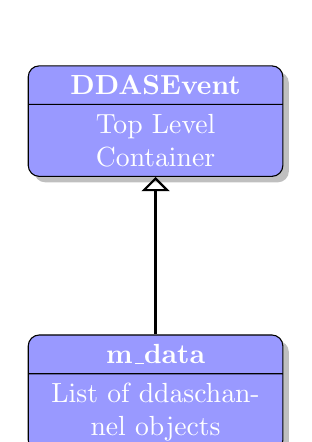
\begin{tikzpicture}[node distance=2cm]
	
	\node (DDASEvent) [abstract, rectangle split, rectangle split parts=2]
        {
            \textbf{DDASEvent}
            \nodepart{second}Top Level Container
        };
	
	\node (mdata) [abstract, rectangle split, rectangle split parts=2, below=of DDASEvent]
        {
            \textbf{m\textunderscore data}
            \nodepart{second}List of ddaschannel objects
        };	



\draw[myarrow] (mdata.north) --++(0,0.3) -| (DDASEvent.south);

\end{tikzpicture}
\end{center}
\caption{Structure of the DDASEvent Class}
\label{fig: DDASEventFig}
\end{figure}


On the S800 side the data is stored in S800 objects (from grROOT).  It contains uncalibrated S800 data.  It does not have things like CRDC xy positions.  See figure \ref{fig: S800Fig} below.  Each S800 object has 6 different major sub objects that hold the information from the different parts of the S800.  For instance to get the first scintillator information one would do:
\example{myS800-$>$GetScintillator(0)-$>$GetDE$\_$up()}

\begin{figure}[h]
\begin{center}
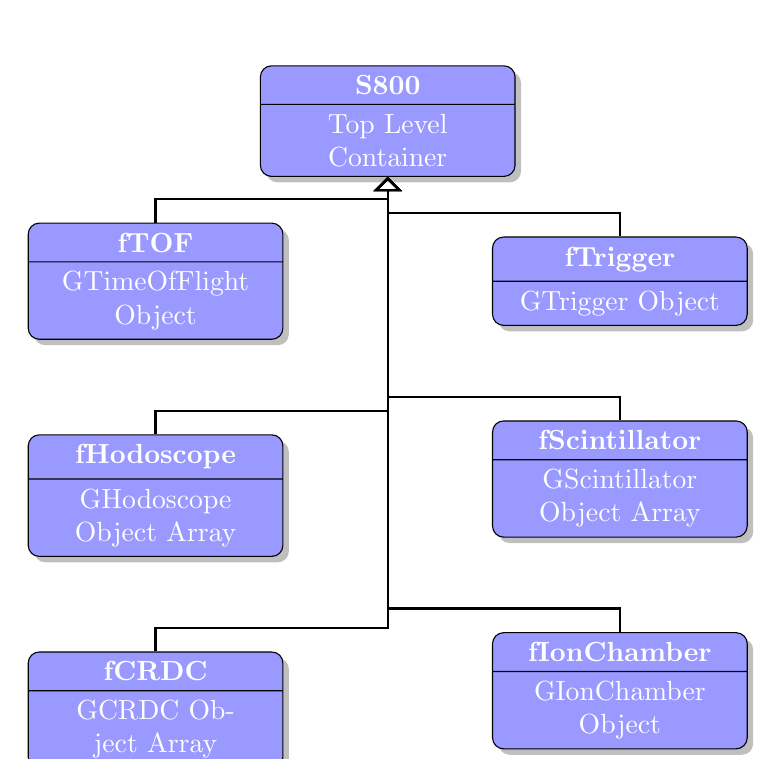
\begin{tikzpicture}[node distance=1.2cm]
	
	\node (S800) [abstract, rectangle split, rectangle split parts=2]
        {
            \textbf{S800}
            \nodepart{second}Top Level Container
        };
	\node (AuxNode01) [text width=0cm, below=of S800] {};	

	\node (fTOF) [abstract, rectangle split, rectangle split parts=2, left=of AuxNode01]
        {
            \textbf{fTOF}
            \nodepart{second}GTimeOfFlight Object
        };	


	
	\node (fHodoscope) [abstract, rectangle split, rectangle split parts=2, below=of fTOF]
        {
            \textbf{fHodoscope}
            \nodepart{second}GHodoscope Object Array
        };	

	\node (fCRDC) [abstract, rectangle split, rectangle split parts=2, below=of fHodoscope]
        {
            \textbf{fCRDC}
            \nodepart{second}GCRDC Object Array
        };	


	\node (fTrigger) [abstract, rectangle split, rectangle split parts=2, right=of AuxNode01]
        {
            \textbf{fTrigger}
            \nodepart{second}GTrigger Object
        };	


	\node (fScintillator) [abstract, rectangle split, rectangle split parts=2, below=of fTrigger]
        {
            \textbf{fScintillator}
            \nodepart{second}GScintillator Object Array
        };	

	\node (fIonChamber) [abstract, rectangle split, rectangle split parts=2, below=of fScintillator]
        {
            \textbf{fIonChamber}
            \nodepart{second}GIonChamber Object
        };	



\draw[myarrow] (fTOF.north) --++(0,0.3) -| (S800.south);
\draw[myarrow] (fHodoscope.north) --++(0,0.3) -| (S800.south);
\draw[myarrow] (fCRDC.north) --++(0,0.3) -| (S800.south);

\draw[myarrow] (fTrigger.north) --++(0,0.3) -| (S800.south);
\draw[myarrow] (fScintillator.north) --++(0,0.3) -| (S800.south);
\draw[myarrow] (fIonChamber.north) --++(0,0.3) -| (S800.south);


\end{tikzpicture}
\end{center}
\caption{S800 Class Structure}
\label{fig: S800Fig}
\end{figure}





























\subsection{Calibrated ROOT Files}

The calibrated ROOT trees are more complicated.  On the S800 side it will be stored as S800calc objects (also from grROOT) where you have provided calibration files to make calibrated energies, times and CRDC xy positions.  See figure \ref{fig: S800calcFig} below.  The structure is similar to the raw S800 objects except that the names are slightly different and they have the calibrated numbers.  For example to get information from the first scintillator:

\example{myS800Calc-$>$GetSCINT(0)-$>$GetDEdown()}



\begin{figure}[h]
\begin{center}
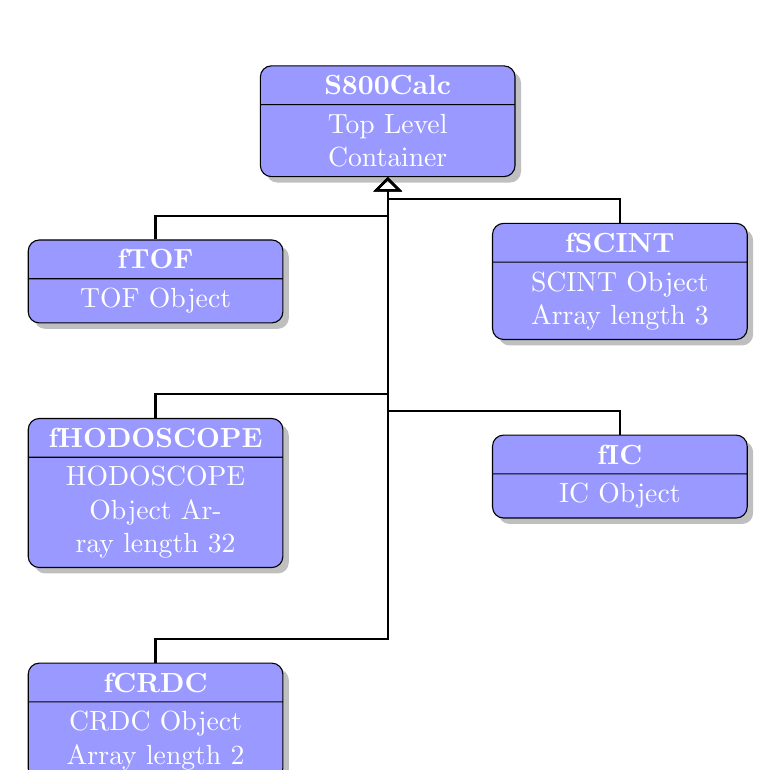
\begin{tikzpicture}[node distance=1.2cm]
	
	\node (S800) [abstract, rectangle split, rectangle split parts=2]
        {
            \textbf{S800Calc}
            \nodepart{second}Top Level Container
        };
	\node (AuxNode01) [text width=0cm, below=of S800] {};	

	\node (fTOF) [abstract, rectangle split, rectangle split parts=2, left=of AuxNode01]
        {
            \textbf{fTOF}
            \nodepart{second}TOF Object
        };	


	
	\node (fHodoscope) [abstract, rectangle split, rectangle split parts=2, below=of fTOF]
        {
            \textbf{fHODOSCOPE}
            \nodepart{second}HODOSCOPE Object Array length 32
        };	

	\node (fCRDC) [abstract, rectangle split, rectangle split parts=2, below=of fHodoscope]
        {
            \textbf{fCRDC}
            \nodepart{second}CRDC Object Array length 2
        };	


	\node (fScintillator) [abstract, rectangle split, rectangle split parts=2, right=of AuxNode01]
        {
            \textbf{fSCINT}
            \nodepart{second}SCINT Object Array length 3
        };	

	\node (fIonChamber) [abstract, rectangle split, rectangle split parts=2, below=of fScintillator]
        {
            \textbf{fIC}
            \nodepart{second}IC Object
        };	



\draw[myarrow] (fTOF.north) --++(0,0.3) -| (S800.south);
\draw[myarrow] (fHodoscope.north) --++(0,0.3) -| (S800.south);
\draw[myarrow] (fCRDC.north) --++(0,0.3) -| (S800.south);


\draw[myarrow] (fScintillator.north) --++(0,0.3) -| (S800.south);
\draw[myarrow] (fIonChamber.north) --++(0,0.3) -| (S800.south);


\end{tikzpicture}
\end{center}
\caption{S800Calc Class Structure}
\label{fig: S800calcFig}
\end{figure}









On the DDAS side it will also make calibrated energies and offset corrected times in the form of LendaEvent objects.  Further, it will take a cable map file and associate together the different channels that fired into bars.  It will also preform the wave form analysis for the different off-line timing algorithms and store each of them in the event.  See figure \ref{fig: LendaEventFig} below.  Each LendaEvent has a variable sized array (std::vector) of LendaBar objects, which contain two variable sized arrays for top and bottom firings.  The top and bottom arrays contain LendaChannel objects.  The LendaChannel objects contain the raw information for a DDAS channel.  The object scintillators are treated differently from the bar channels.  They are stored in a variable sized array of LendaChannels in the LendaEvent called TheObjectScintillators.  If there was an event with 1 bar you can access the energy of the top channel (from pulse integration) with:
\example{myLendaEvent-$>$Bars[0].Tops[0].GetEnergy()}

If the event had one bar with 2 top channel firings (a pile up event) the second firing could be accessed with:
\example{myLendaEvent-$>$Bars[0].Tops[1].GetEnergy()}






\begin{figure}[h]
\begin{center}

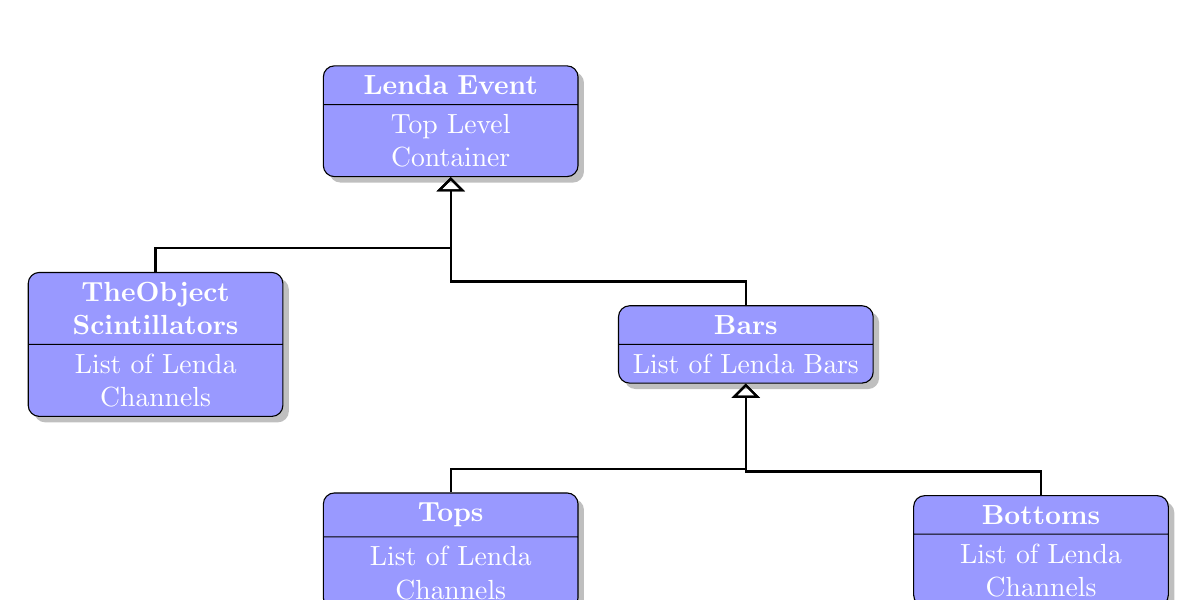
\begin{tikzpicture}[node distance=2cm]
	
	\node (LendaEvent) [abstract, rectangle split, rectangle split parts=2]
        {
            \textbf{Lenda Event}
            \nodepart{second}Top Level Container
        };
	\node (AuxNode01) [text width=0cm, below=of LendaEvent] {};

	\node (ObjectScintillators) [abstract, rectangle split, rectangle split parts=2, left=of AuxNode01]
        {
            \textbf{TheObject Scintillators}
            \nodepart{second}List of Lenda Channels
        };	

\node (Bars) [abstract, rectangle split, rectangle split parts=2, right=of AuxNode01]
        {
            \textbf{Bars}
            \nodepart{second}List of Lenda Bars
        };	
	\node (AuxNode02) [text width=0cm, below=of Bars] {};

\node (Tops) [abstract, rectangle split, rectangle split parts=2, left=of AuxNode02]
	{
	\textbf{Tops}
 	\nodepart{second}List of Lenda Channels
	};
\node (Bottoms) [abstract, rectangle split, rectangle split parts=2, right=of AuxNode02]
	{
	\textbf{Bottoms}
 	\nodepart{second}List of Lenda Channels
	};


\draw[myarrow] (ObjectScintillators.north) --++(0,0.3) -| (LendaEvent.south);
\draw[myarrow] (Bars.north) --++(0,0.3) -| (LendaEvent.south);
\draw[myarrow] (Tops.north) --++(0,0.3) -| (Bars.south);
\draw[myarrow] (Bottoms.north) --++(0,0.3) -| (Bars.south);
\end{tikzpicture}
\end{center}
\caption{LendaEvent Class Structure}
\label{fig: LendaEventFig}
\end{figure}
















\section{R00TLe Users}
\label{sec:R00TLe users}

Making a "user" in R00TLe simply means having a directory in the R00TLeInstall/users/ directory.  This is done by using the R00TLeLogon.sh script.  The first time you logon as a new user use:
\example{R00TLeLogon.sh -f AUserName}



Afterwards simply

\example{R00TLeLogon.sh AUserName}

Logging on as a user will do several things.  Firstly, it will bring you to an independent working area where you can do analysis without affecting other users.  Further, in your directory it will generate startup files for ROOT so that your sessions have access to all the R00TLe libraries.  In particular a .rootrc file and a rootlogon.C file will be generated.  These will setup your ROOT sessions (only when you execute ROOT from your user's directory) so that the S800 and LENDA libraries are preloaded. It will also make symbolic links to the directories containing the evt and ROOT files that were specified at install time.  This way you can access the files built with R00TLe easily with:
\example{root rootfiles/run-0001-00.root}

The other main thing that the R00TLeLogon.sh script does is copy over the skeleton histogram-er into your directory (the first time it is executed).  It consists of three directories:
\begin{enumerate}
\item macros: A local directory for the user to put ROOT macros in
\item src: The directory where the Analoop program is (the histogram dumper)
\item histograms: The directory where Analoop puts your histogram files
\end{enumerate}

To analyze a run (that has already been built into a calibrated tree) you can simply do the following from a ROOT session:
\example{.x main.C(TheRunNumber)}

main.C is a ROOT macro (it is copied over into the macros directory at login) that will load the R00T file for the given run, then compile your Analoop program and then run Analoop over the file.  See the example section \ref{sec: Using the Skeleton Histogram Dumper} for more details.













\section{Examples}
\label{sec: examples}


\subsection{Accessing information in the Interpreter}

In this example the syntax for making a histogram from within the ROOT interpreter is shown.  It will use calibrated ROOT file run-0399-00.root, which was one of the test beam runs. First log in to your R00TLe directory:
\example{R00TLeLogon.sh sam}
Then open the root file with:
\example{$<$pike:sam$>$ root rootfiles/run-0398-00.root}

To list the contents of the ROOT file type:
\example{.ls}
You should see something like the following:
\begin{verbatim}
TFile**         rootfiles/run-0398-00.root
 TFile*         rootfiles/run-0398-00.root
  KEY: TTree    caltree;1       S800 and DDAS calibrated events
  KEY: R00TLeSettings   TheSettings;1   R00TLe's Settings
\end{verbatim}

The file contains a ROOT tree named caltree and a settings object called TheSettings.  Histograms can be drawn from the tree with the draw command.  It has the syntax:

\example{caltree-$>$Draw("variable selection","cuts","graphics options");}

\subsubsection{DDAS Side}
So to draw the energy spectrum for the top PMT from one of the LendaChannels you would have the following:
\MultiBox{caltree->Draw("lendaevent.Bars[0].Tops[0].GetEnergy()",\\
"lendaeavent.NumBars==1$\&\&$lendaevent.Bars[0].SimpleEventBit$\&\&$\\
lendaevent.Bars[0].BarId==2")}


\MultiBox{Note:  I like my software overly long and wordy}

\Graph{EnergyPicForDocumentationFrom398.png}{What the histogram should look like}
Figure \ref{fig: EnergyPicForDocumentationFrom398.png} shows what this draw command should look like in from run 398.

To break down this command the first argument:
\example{"lendaevent.Bars[0].Tops[0].GetEnergy()"}

calls for the first top firing in the first bar in the event and gets the energy.  The second argument has three different cuts to the data. First:
\example{lendaeavent.NumBars==1}

only plot from events with one bar.  Second:
\example{lendaevent.Bars[0].SimpleEventBit}

requires that the first bar in the event (and only bar due to condition one) is a "simple event".  A Simple Event in this context means that there was no crazy pile up.  I.e. the event had exactly one top and one bottom.  The third condition:
\example{lendaevent.Bars[0].BarId==2}
selects which of the 48 bars you are interested in.  During the building of the calibrated root file each bar is given an unique bar id.  In this case we are selecting number 2.  If you don't remember which bar is what, you can ask the settings object (which has saved all the information from the building process).  In this case BarId 2 corresponds to SL03.

\MultiBox{root [2] TheSettings-$>$GetBarName(2)\\
(class TString)"SL03"
}



\subsubsection{S800 Side}

Making histograms of s800 data is done in a similar fashion.  As an example we will plot the sum energy from the IC (also from run 398).
\MultiBox{caltree-$>$Draw("s800calc.GetIC().GetSum()")}

Here we are making no cuts so there is not second argument.  The result of this plot can be seen in figure \ref{fig: S800ICSumForDocumenationFrom398.png}.  Plots containing  both S800 and DDAS data can also be made with a draw command.

\Graph{S800ICSumForDocumenationFrom398.png}{S800 IC Sum example}

\MultiBox{caltree-$>$Draw("s800calc.GetIC().GetSum():lendaevent.Bars[0].Tops[0].GetEnergy()",\\
"lendaeavent.NumBars==1$\&\&$lendaevent.Bars[0].SimpleEventBit$\&\&$\\
lendaevent.Bars[0].BarId==2")}

Here we have the S800 ion chamber sum plotted against the energy in the top PMT of Lenda Bar 2.  It has the same cuts as the above Lenda examples.

\subsubsection{Complicated Draw Commands}
Below are some more examples of ever more complicated draw commands with explanations on what they mean.
\\ \\
Below will plot the 2-D histogram of center of gravity vs top-bottom time difference in bar 2.  It has the same restrictions on multiplicity as the above example.
\MultiBox{caltree-$>$Draw("lendaevent.Bars[0].GetCOG():lendaevent.Bars[0].GetDt()",\\
"lendaevent.NumBars==1$\&\&$lendaevent.Bars[0].SimpleEventBit$\&\&$\\lendaevent.Bars[0].BarId==2")}


Below will plot the 1-D histogram of the top channels time of flight.  I.e. the timestamp of the top PMT channel minus the timestamp of the top PMTs reference time (as defined in the map file).  Like Above it still has the same multplicity cuts in it and still selects bar ID equal to 2.
\MultiBox{caltree-$>$Draw("lendaevent.Bars[0].GetTopTOF()",\\
"lendaevent.NumBars==1$\&\&$lendaevent.Bars[0].SimpleEventBit$\&\&$\\lendaevent.Bars[0].BarId==2")}

Below will produce the same 1-D histogram as above.  The time of flight for the top PMT channel.  For some quantities the events store redundant information.  The LendaBar class will calculate and store the time of flight, but the raw information is still stored in the underlying LendaChannels.  Most of the quantities that LendaBar calculates are for convenience (like TOF, average energy, average time...).
\MultiBox{caltree-$>$Draw("lendaevent-$>$Bars[0].Tops[0].GetTime()-\\lendaevent-$>$Bars[0].Tops[0].GetReferenceTime()",\\
"lendaevent.NumBars==1$\&\&$lendaevent.Bars[0].SimpleEventBit$\&\&$\\lendaevent.Bars[0].BarId==2")}



\subsection{Using the Skeleton Histogram Dumper}
\label{sec: Using the Skeleton Histogram Dumper}

The generic histogram dumper, that is copied to each user directory when it is created, consists of three files: main.C, Analoop.cc and Analoop.h.
\subsubsection{main.C}
Main.C is a wrapper script to make calling running the Analoop program simpler.  It can be called in the following ways:
\begin{enumerate}
\item .x main.C : when no arguments are given it will load the files that are hard coded into the script.  When it is done dumping those files it will save them in the histograms directory as temp.root.
\item .x main.C(RunNum) : when a run number argument is given it will look for files called "rootfiles/run-RunNum-??.root" if it finds them it will run Analoop and save the result in the histograms directory as HistogramsFromRun$\#\#\#\#$.root
\item .x main.C(RunNum,AFileName) : when two arguments are given you can specify an output file name.  Instead of saving the histograms as HistogramsFromRun$\#\#\#\#$.root it will save them as the given file name.
\end{enumerate}

\subsubsection{Analoop}

The Analoop program is the bit of code that actually making the histograms.  Technically it defines a "TSelector" object, which a ROOT class designed to loop over ROOT trees and make histograms.  Doing it this way makes the syntax slightly more cumbersome but allows for the use  of PROOF (the parallel ROOT facility).  Analoop has two parts a header file and a source file:
\begin{enumerate}
\item Analoop.h is the header file.  This is where you would declare but not initialize histograms. I.e. you would say something like:
\example{TH1F * MyHistogram}
but \textbf{not}
\example{ TH1F *MyHistogram = new TH1F("MyHistogram","Title",nBins,xLow,xHigh)}
\item Analoop.cc is the source file.  This where you "new" the histograms and where you make cuts and fill histograms.  See below for details.
\end{enumerate}

The places in the code where you make changes are clearly commented.    There are two ways to make histograms in Analoop.  The more direct and cumbersome way is to declare the histogram in the header file, allocate it in \textit{SlaveBegin} and fill it in \textit{Process}.  Doing it this way means that you will have to change the header file as above and add lines in the source file.  This is explained in detail below and will be refered to as method 1.  The other way is to use the \textit{AutoHisto} commands, which will allow you to declare and fill a histogram in one line in the \textit{Process} function without changing the header file.  This is also explained below and will be refered to as method 2.


\subsubsection{Analoop.cc in detail}

Since Analoop.cc is where the real physics analysis will occur it is important to go into some details.  There are two important functions defined (they are the first two in the file and are commented): SlaveBegin and Process.  Slave begin is called once at the start of the program.  It is where histograms are allocated in method 1.  In SlaveBegin there is already some code that allocates histograms for standard Lenda quantities for all the bars (TOFs, PulseHeights...).  This is done under the comment that says
\example{Make histograms for standard quantities  (TOFs and PulseHeights).}

Below that is another comment specifying a good place to "new" more histograms that you have declared in the header.  This is where you would say some thing like:
\example{MyHistogram = new TH1F("MyHistogram","Title",100,-10,10)}

The second important function is Process.  This function is called for each entry in the ROOT tree (each event) and is where the filling of histograms is done.  There is already code in there to fill the "standard Lenda quantities".  It has the general structure: \\



\begin{lstlisting}
 for (int i =0;i<NumBarsInEvent;i++){ //Loop over all Bars in the Lenda event
    int NumTopsInBar = lendaevent->Bars[i].NumTops;
    int NumBottomsInBar = lendaevent->Bars[i].NumBottoms;
    int BarId = lendaevent->Bars[i].BarId; //The ith Bars Unique Bar Id

    for (int t=0;t<NumTopsInBar;t++){ // Loop over all the TOPS in the Bar
    	TopEnergies[BarId]->Fill(E);
    	//Do stuff for Tops
    }//End for over tops

    for (int b=0;b<NumBottomsInBar;b++){//Loop over all the Bottoms in the Bar
    	BottomEnergies[BarId]->Fill(E);
   	//Do Stuff For bottoms
    }//End for over bottoms

    if (lendaevent->Bars[i].SimpleEventBit){//has 1 top and 1 bottom
    	AvgTOFs[BarId]->Fill(lendaevent->Bars[i].GetAvgTOF());
    }
}//End Loop Over Bars
\end{lstlisting}

Here we see that for each entry in the tree the Lenda information can be accessed through the lendaevent pointer.  In order to extract all the channel firings from the Lenda event, one must loop over all bars and for each bar all tops and all bottoms.  This is what is done above.  As an example of how to add code to this structure (still using method 1) we will fill our example histogram with the top bottom time difference for bar south Lenda 5 (SL05).  Here is the same code again with the added lines:

\begin{lstlisting}
 for (int i =0;i<NumBarsInEvent;i++){ //Loop over all Bars in the Lenda event
    int NumTopsInBar = lendaevent->Bars[i].NumTops;
    int NumBottomsInBar = lendaevent->Bars[i].NumBottoms;
    int BarId = lendaevent->Bars[i].BarId; //The ith Bars Unique Bar Id

	for (int t=0;t<NumTopsInBar;t++){ // Loop over all the TOPS in the Bar
		TopEnergies[BarId]->Fill(E);
		//Do stuff for Tops
	}//End for over tops

	for (int b=0;b<NumBottomsInBar;b++){//Loop over all the Bottoms in the Bar
		BottomEnergies[BarId]->Fill(E);
		//Do Stuff For bottoms
	}//End for over bottoms

	if (lendaevent->Bars[i].SimpleEventBit){//has 1 top and 1 bottom
		AvgTOFs[BarId]->Fill(lendaevent->Bars[i].GetAvgTOF());
		//Can only have top bottom time difference for 1 top and 1 bottom
		if (lendaevent->Bars[i].Name=="SL05"){                  //NEW LINE
			MyHistogram->Fill(lendaevent->Bars[i].GetDt());   //NEW LINE
		}
	}
}//End Loop Over Bars
\end{lstlisting}

We can preform the same operation with the \textit{AutoHisto} method (method 2).  For this method we don't need to new the histogram in \textit{SlaveBegin} and we don't need to declear it in the header file.  We need only call \textit{AutoHisto} in the process function:

\example{AutoHisto("name",value,nBins,xlow,xhigh)}

The first time process is called the histogram will be created and filled automatically.  Subsequent times the histogram will be found and filled again.  NOTE! This method can come at a performance loss.  Below is what the code will look like to fill the top bottom time difference for south Lenda 5 with \textit{AutoHisto}:

\begin{lstlisting}
 for (int i =0;i<NumBarsInEvent;i++){ //Loop over all Bars in the Lenda event
    int NumTopsInBar = lendaevent->Bars[i].NumTops;
    int NumBottomsInBar = lendaevent->Bars[i].NumBottoms;
    int BarId = lendaevent->Bars[i].BarId; //The ith Bars Unique Bar Id

	for (int t=0;t<NumTopsInBar;t++){ // Loop over all the TOPS in the Bar
		TopEnergies[BarId]->Fill(E);
		//Do stuff for Tops
	}//End for over tops

	for (int b=0;b<NumBottomsInBar;b++){//Loop over all the Bottoms in the Bar
		BottomEnergies[BarId]->Fill(E);
		//Do Stuff For bottoms
	}//End for over bottoms

	if (lendaevent->Bars[i].SimpleEventBit){//has 1 top and 1 bottom
		AvgTOFs[BarId]->Fill(lendaevent->Bars[i].GetAvgTOF());
		//Can only have top bottom time difference for 1 top and 1 bottom
		if (lendaevent->Bars[i].Name=="SL05"){
			AutoHisto("MyHistogram",lendaevent->Bars[i].GetDt(),100,-10,10);
		}
	}
}//End Loop Over Bars
\end{lstlisting}



\subsection{From Evt file to Histogram file}

In this example the whole process for processing data is shown step by step.  For this example run 394 will be used (this was one of the runs from the summer 2014 test beam).

\begin{enumerate}
\item Log on to R00TLe user
\example{R00TLeLogon.sh sam}
This should output:
\MultiBox{
Setting environment Variables\\
User sam found.\\
Switching to working directory...\\
Generating ROOT start up file...\\
Generating ROOT logon file...\\
Found histogrmer already.  Won't over write\\
}

\item Build Raw ROOT file
\example{BuildRaw.sh 394}
This should output something like:
\MultiBox{
Build Raw Root File\\
Info in \ls Evt2Raw\gr : Input file:  ./evtfiles/run-0394-00.evt\\
Info in \ls Evt2Raw\gr : Input file size:  124.79 MB\\
Info in \ls Evt2Raw\gr : Output file: ./rootfiles/run-0394-00-RAW.root\\
Info in \ls Evt2Raw\gr : Total of 37686 data buffers (124.79 MB read)636.91 buffers/sec...   1.16 sec to go\\
Info in \ls Evt2Raw\gr : Total of 34864 raw events written\\
Info in \ls Evt2Raw\gr : Decoded 6786.683594 buffers/sec.\\
Real time 0:00:05.552930, CP time 4.680\\
}


\item Build Calibrated ROOT file:
\example{BuildData.sh 394}

Assuming that you have provided appropriate DDAS map and corrections files and S800 calibration files this will build the calibrated trees.  You should see an output like:

\MultiBox{
Build From Raw Root\\
Info in \ls Raw2Cal\gr : Input file:  ./rootfiles/run-0394-00-RAW.root\\
Info in \ls Raw2Cal\gr : Input file size:   74.85 MB\\
Info in \ls Raw2Cal\gr : 34864 entries in the input file\\
Info in \ls Raw2Cal\gr : Output file: ././rootfiles/run-0394-00.root\\
Info in \ls LendaPacker\gr : Using MapFile MapFile.txt and CorrectionsFile Corrections394.txt\\
Info in \ls Raw2Cal\gr : Reading a parameter file /user/lipschut/R00TLe/prm/Raw2Cal.prm\\
Real time 0:01:37.661684, CP time 43.450=================]\\
}


\item Open ROOT
\example{root}

\item run the histogram dumper on run 394
\example{.x main.C(394)}

This should output

\begin{verbatim}
Creating TChain... Done.
List of files:
Collection name='TObjArray', class='TObjArray', size=100
 OBJ: TChainElement     caltree ./rootfiles/run-0394-00.root
Info in <TUnixSystem::ACLiC>: creating shared library /user/lipschut/R00TLe/-
users/sam/src/Analoop_cc.so
Info in <Analoop::Notify>: File: ./rootfiles/run-0394-00.root ( 147.13 MB)
Info in <Analoop::Notify>: 34864 entries (100.00%) in this tree
Info in <Analoop::Notify>: 34864 entries (100.00%) up to this tree
File will be saved in /user/lipschut/R00TLe/users/bob/histograms/-
HistogramsFromRun394.root
Info in <WriteHist>: Histograms have been written to /user/lipschut/R00TLe/-
users/sam/histograms/HistogramsFromRun394.root
Info in <Analoop::Analoop>: Destructing.
\end{verbatim}

After this there will be a HistogramsFromRun394.root file in the local histograms directory that contains the default histograms

\end{enumerate}










\end{document}


